% Preliminary notes:
% To be compiled this document require the definition of multiple macros
% - \greyed :: Defines how to treat text from part which were part of the FIFA
%              rules but have been suspended for the RoboCup Rulebook
% - \simplify :: Roughly similar to '\greyed' difference is not explicit
% - \removed :: How to display text which has been removed since last edition,
%               this command should not be used on 'items' from list or for
%               entire sections of the document, but only inside paragraphs.
%               It can affects how text is displayed (e.g. strikethrough).
% - \removedSection :: Signals portions of the text which need to be removed
%                      from the text in the shorten version. It can be used
%                      inside of itemize or contain itemize environments and
%                      only control visibility of the elements.
% - \added :: is used to signal that text has been changed since last version.
%             Controls the color of the text if changes are marked.

\documentclass[a4paper]{article}

\usepackage[utf8]{inputenc}
\usepackage[T1]{fontenc}
\usepackage[english]{babel}
\usepackage{amsmath}
\usepackage{amssymb,amsfonts,textcomp}
\usepackage{color}
\usepackage{array}
\usepackage{supertabular}
\usepackage{hhline}
\usepackage{hyperref}
\usepackage{tocbibind}
\usepackage{subcaption}
\usepackage[normalem]{ulem}
\newcommand{\rulesauthor}{Comitê Técnico RoboCup Brasil Humanoid}
\hypersetup{
    colorlinks=true, linkcolor=blue, citecolor=blue, filecolor=blue, urlcolor=[rgb]{0,0,0.5},
    pdftitle=, pdfauthor=\rulesauthor, pdfsubject=, pdfkeywords=
}
\usepackage[pdftex]{graphicx}
\usepackage{adjustbox}

\usepackage{tikz}
\usetikzlibrary{backgrounds,arrows,calc,math,positioning,shapes, decorations.markings,decorations.pathreplacing}

\makeatletter
\newcommand\arraybslash{\let\\\@arraycr}
\makeatother
\usepackage{tikz}
\usetikzlibrary{backgrounds,arrows,calc,math,positioning,shapes, decorations.markings,decorations.pathreplacing}

% Page layout (geometry)
\usepackage[modulo]{lineno}
\linenumbers

\newcommand\headlinebox{
    \vspace{-0.1cm}
    \fbox{\rule{6.6in}{0pt}\rule[-0.05ex]{0pt}{0.05ex}}
    \vspace{0.1cm}
}

\setlength\voffset{-1in}
\setlength\hoffset{-1in}
\setlength\topmargin{0.7874in}
\setlength\oddsidemargin{0.7874in}
\setlength\textheight{9.754932in}
\setlength\textwidth{6.6932993in}
\setlength\footskip{26.148pt}
\setlength\headheight{0cm}
\setlength\headsep{0cm}
% Footnote rule
\setlength{\skip\footins}{0.0469in}
\renewcommand\footnoterule{\vspace*{-0.0071in}\setlength\leftskip{0pt}\setlength\rightskip{0pt plus 1fil}\noindent\textcolor{black}{\rule{0.25\columnwidth}{0.0071in}}\vspace*{0.0398in}}
\setlength\parindent{0pt}
% Pages styles
\makeatletter
\newcommand\ps@Standard{
    \renewcommand\@oddhead{}
    \renewcommand\@evenhead{}
    \renewcommand\@oddfoot{\thepage{}}
    \renewcommand\@evenfoot{\@oddfoot}
    \renewcommand\thepage{\arabic{page}\texorpdfstring{\hfill}{}}
}
\makeatother
\pagestyle{Standard}
\setlength\tabcolsep{1mm}
\renewcommand\arraystretch{1.3}
\title{}
\author{\rulesauthor}
\date{2024-06-26}

% Redefinir o nome da figura
\captionsetup[figure]{name=Figura}

\begin{document}
    \sffamily

    \begin{center}
        
\includegraphics[height=0.9055in]{img/robocup_logo.jpg}

        {\Huge \bfseries
        RoboCup Brasil
        \\
        Humanoid League -  Entry Level
        \\
        Regras do Jogo
        \\ \vspace{0.5cm}
        2024}

        \bigskip

        {\bfseries 26 Jun, 2024}
    \end{center}

    \begin{figure}[!h]
        \centering
        \adjustbox{trim=2.5cm 0cm 5cm 3cm,clip}
        {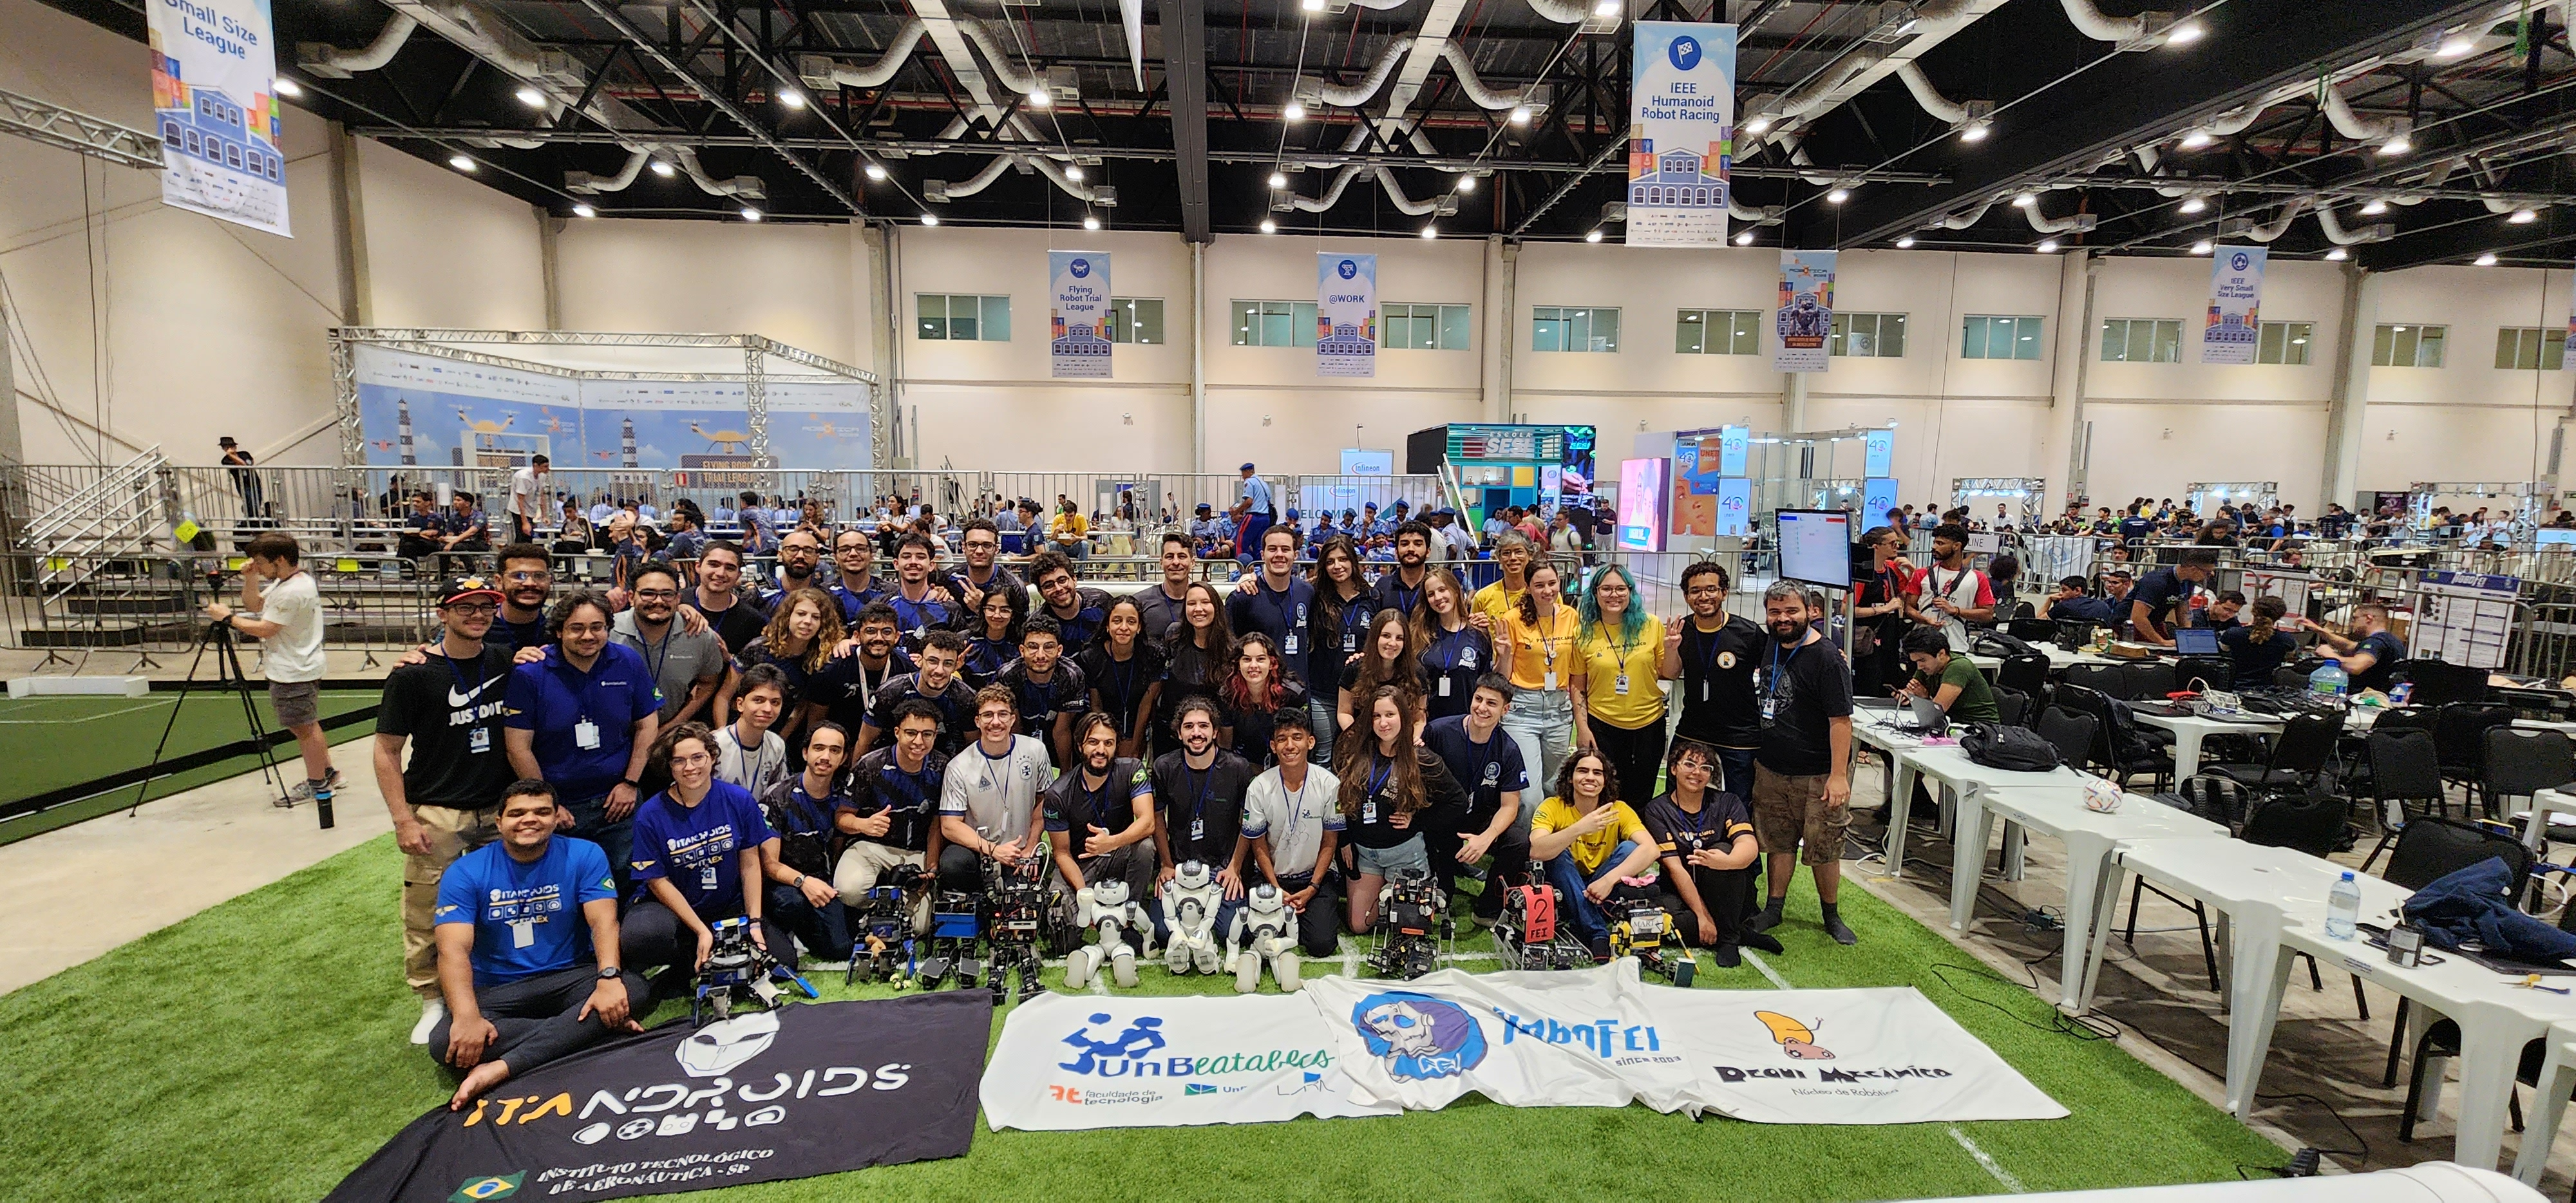
\includegraphics[height=4in]{img/cover_2023.jpg}}
        \captionsetup{labelformat=empty}
        \caption{A foto do grupo da liga humanóide de 2023}
    \end{figure}

    % \removedSection{
    %     \large As alterações no livro de regras do ano passado são \added{marcadas em magenta cor do texto} (para acréscimos) ou por \removed{texto riscado} (para exclusões)
    % }

    \bigskip
    RoboCup Brasil (para anúncios importantes):\\
    \url{https://cbr.robocup.org.br}

    \medskip
    Chair: Vinicius Ferreira (para discussão de regras e perguntas):\\
    vinicius.nicassio@gmail.com

    % \medskip
    % RoboCup Humanoid League Home Pages:\\
    % \url{https://www.humanoid.robocup.org/}\\
    % \url{https://www.robocup.org/leagues/3}

    \medskip
    Inspirado em \href{https://github.com/RoboCup-Humanoid-TC/Rules}{\textcolor[rgb]{0,0,0.5 }{RoboCup Humanoid League TC - Rules}},\\
    com alterações para a RoboCup Brasil.

    \setcounter{figure}{0}

    \clearpage

    {\bfseries\color[rgb]{0.4,0.4,0.4}
    Visão geral}

    \bigskip

    Seção I: Regras da Competição

    \bigskip

    Seção II: Desafios
    
    \bigskip

    Seção III: Desafios de Visão

    \bigskip

    Seção IV: Desafios de Controle
    
    \bigskip

    Seção V: Desafios de Comunicação

    \clearpage

    {\bfseries\color[rgb]{0.4,0.4,0.4}
    Sumário}

    \addtocontents{toc}{\protect\setcounter{tocdepth}{0}}
    \renewcommand\contentsname{}
    \vspace*{-1cm}
    \tableofcontents
    \addtocontents{toc}{\protect\setcounter{tocdepth}{2}}


%%%%%%%%%%%%%%%%%%%%%%%%%%%%%%%%%%%%%%%%%%%
%%%%%%%%%%% SECTION I %%%%%%%%%%%%%%%%%%%%%
%%%%%%%%%%%%%%%%%%%%%%%%%%%%%%%%%%%%%%%%%%%

    \clearpage

    \begin{center}
        \Huge\bfseries{
            \vspace*{3cm}
            Seção I

            \vspace*{2cm}

            Regras da Competição}
    \end{center}
    \addcontentsline{toc}{section}{Seção I: Regras da Competição}

    \vspace*{12cm}

    % As Leis do Jogo devem ser atualizadas regularmente para se referirem ao documento mais recente da FIFA.

    % \bigskip

    % \simplify{
    %     Os desvios das regras da FIFA estão marcados no texto:

    %     \bigskip
    %     \begin{tabular}{ll}
    %         'substitui': &Uma regra específica do RoboCup substitui temporariamente uma regra da FIFA.\\
    %         'suspenso': &Uma regra específica da FIFA ainda não foi aplicada.\\
    %         'novo': &Uma regra específica do RoboCup é introduzida temporariamente.
    %     \end{tabular}
    % }

    \clearpage
\sffamily
{\bfseries\color[rgb]{0.4,0.4,0.4}
NOTAS SOBRE AS LEIS DO JOGO}

\bigskip

{\color[rgb]{0.4,0.4,0.4}{Modificações} }

Sujeito ao acordo das equipes participantes e desde que os princípios destas regras sejam mantidos, as regras podem ser modificadas na sua aplicação para os desafios.

Qualquer uma ou todas as seguintes modificações são permitidas:

\begin{itemize}
  \item Tamanho do campo onde os desafios serão realizados
  \item Tamanho, peso e material utilizados nos desafios
  \item Largura entre os postes e altura da trave em relação ao solo
  \item Duração do períodos dos desafios
  \item Penalizações
  \item Pontuações
\end{itemize}

\bigskip

{\color[rgb]{0.4,0.4,0.4}{Línguas oficiais}}

O Comitê Técnico da RoboCup Brasil publica as regras do jogo em português do Brasil. Caso uma equipe necessite, uma versão em inglês pode ser fornecida.

% \simplify{
%   \bigskip

%   {\color[rgb]{0.4,0.4,0.4}{Chave} }
%   Uma única linha na margem esquerda indica novas alterações na lei.
% }

    \clearpage

    \clearpage
\sffamily
{\bfseries\color[rgb]{0.4,0.4,0.4}
Regra 1 – O Campo dos Desafios}
\phantomsection
\addcontentsline{toc}{subsection}{Regra 1 – O Campo dos Desafios}

\bigskip
{\bfseries Superfície do campo}

\headlinebox
Os desafios serão executados no mesmo campo da competição RoboCup Brasil Humanoid Soccer League, cuja superfície é de grama artificial com altura aproximada de 30 mm.

\bigskip

(Modificações: Caso os organizadores locais não consigam encontrar uma grama com altura aproximada de 30 mm, uma grama com altura menor pode ser utilizada sem aviso prévio às equipes.)

\bigskip
{\sffamily
A cor das superfícies artificiais deve ser verde.}

\bigskip
{\bfseries
Marcações de campo}

\headlinebox

O campo de jogo deve ser retangular e marcado com linhas. Essas linhas pertencem às áreas das quais são limites.

\bigskip

As duas linhas de limite mais longas são chamadas de linhas de toque. As duas linhas mais curtas são chamadas de linhas de gol.

\bigskip

O campo de jogo é dividido em duas metades por uma linha intermediária, que une os pontos médios das duas linhas laterais.

\bigskip

A marca central é indicada no ponto médio da linha intermediária.
Um círculo está marcado ao seu redor.

\bigskip

{\textbf{Dimensões}}

\headlinebox

As dimenções do campo estão descritos na \href{https://cbr.robocup.org.br/wp-content/uploads/2024/04/LARC2024.pdf}{\textcolor[rgb]{0,0,0.5 }{Regra da Competição da RoboCup Brasil Humanoid Soccer League}}.
    \clearpage
\sffamily
{\bfseries\color[rgb]{0.4,0.4,0.4}
Regra 2 – As Bolas}
\phantomsection
\addcontentsline{toc}{subsection}{Regra 2 – As Bolas}


\bigskip

{\bfseries Qualidades e medidas }

\headlinebox

As bolas que serão utilizadas para os desafios são as mesmas em competições anteriores da RoboCup Brasil Humanoid League. A bola é:

\begin{itemize}
\item esférica
\item é feito ou se assemelha ao peso, forma, características de movimento e aparência de couro ou outro material adequado
\item FIFA tamanho 1.
\end{itemize}

{\bfseries Substituição de uma bola defeituosa}

\headlinebox

Se a bola estourar ou apresentar defeito durante a partida:

\begin{itemize}
\item o desafio é interrompido
\item um novo desafio é iniciado e a pontuação é zerada
\end{itemize}

A bola não pode ser trocada durante um desafio sem a autorização do avaliador.
    \clearpage
\sffamily

{\bfseries\color[rgb]{0.4,0.4,0.4}
Regra 3 – Os Jogadores}
\phantomsection
\addcontentsline{toc}{subsection}{Regra 3 – Os Jogadores}


\bigskip

{\bfseries Número de jogadores}

\headlinebox

Cada desafio terá um número exato de jogadores, que será descrito posteriormente. No entanto, é necessário que a equipe tenha pelo menos um jogador por desafio, exceto nos desafios que não requerem movimentação. As exceções serão detalhadas em seus respectivos desafios.

\bigskip

{\bfseries Número de substituições}

\headlinebox
 
{\bfseries Competições oficiais }

Durante os desafios, as equipes poderão substituir o jogador até três vezes. A substituição do mesmo jogador, ao sair e entrar novamente em um desafio, contará como duas substituições.

\bigskip

{\bfseries Procedimento de substituição}

\headlinebox

Para substituir um jogador por um substituto, devem ser observadas as seguintes condições:

\begin{itemize}
\item o avaliador deve ser informado antes de qualquer substituição proposta ser feita
\item o desafio será interrompido e a pontuação realizadas até o momento será descartada
\item um novo desafio será iniciado e uma nova pontuação será realizada.
\end{itemize}

% \bigskip

% {\bfseries Infrações e sanções}

% \headlinebox

% Se um substituto ou jogador substituído ou um oficial de equipe entrar no campo de jogo sem a permissão do avaliador:

% \begin{itemize}
% \item the referee stops play (although not immediately if the substitute or substituted player does not interfere with play)
% \item the referee cautions him for unsporting behaviour and orders him to leave the field of play
% \item if the referee has stopped play, it is restarted with an direct free kick
%       for the opposing team from the position of the ball at the time of the
%       stoppage (see rule 13 -- Position of free kick)
% \end{itemize}

% \bigskip

% If a named substitute enters the field of play instead of a named player at the start of the match and the referee is not informed of this change:

% \begin{itemize}
% \item the referee allows the named substitute to continue the match
% \item no disciplinary sanction is taken against the named substitute
% \item the number of substitutions allowed by the offending team is not reduced
% \item the referee reports the incident to the appropriate authorities
% \end{itemize}

% \bigskip

% If a player changes places with the goalkeeper without the
% referee's permission before the change is made:

% \begin{itemize}
% \item the referee allows play to continue
% \item the referee cautions the players concerned when the ball is next out of play
% \end{itemize}

% \bigskip

% In the event of any other infringements of this rule:

% \begin{itemize}
% \item the players concerned are cautioned
% \item the match is restarted with an indirect free kick, to be taken by a player of the opposing team from the position of the ball at the time of the stoppage (see rule 13 -- Position of free kick)
% \end{itemize}
    \clearpage
\sffamily
{\bfseries\color[rgb]{0.4,0.4,0.4}
Regra 4 – Os Jogadores ('Equipamento')}
\phantomsection
\addcontentsline{toc}{subsection}{Regra 4 – Os Jogadores ('Equipamento')}

\bigskip

{\bfseries Segurança }

\headlinebox

Um jogador não deve usar equipamento ou vestir qualquer coisa que seja perigosa para si mesmo ou para outro jogador (incluindo qualquer tipo de joia).

\bigskip

{\bfseries O Design dos Robôs}

\headlinebox

Os robôs participantes das competições da Liga Humanóide devem ter um plano corporal semelhante ao humano, como mostrado na Fig. \ref{fig:bodyplan}. Eles devem consistir em duas pernas, dois braços e uma cabeça, que estão presos a um tronco.

\bigskip

Os robôs devem estar equipados com uma alça, para serem recolhidos com segurança e sem causar danos ao robô e ao manipulador. A alça deve ser facilmente acessível e não deve interferir com a operação do robô.

\begin{figure}[h]
\begin{center}
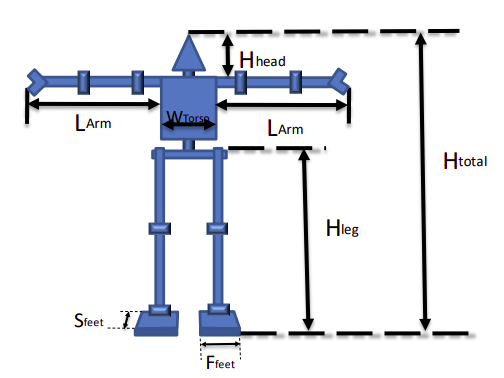
\includegraphics[width=0.7\textwidth]{img/bodyplan.png}
\caption{Exemplo de plano corporal de um robô humanóide}
\label{fig:bodyplan}
\vspace{-3ex}
\end{center}
\end{figure}


Os robôs devem ser capazes de ficar em pé e andar sobre as pernas.
Os únicos modos de locomoção permitidos são andar bípede, correr e saltar.

\bigskip

Todas as ações dos robôs devem ser cinematicamente equivalentes aos movimentos humanóides.

\bigskip

{\bfseries Altura do Robô}

\headlinebox

Com base em $H_{total}$, aplicam-se as seguintes restrições de tamanho:
\begin{itemize}
\item 25 cm ${\leq}$ $H_{total}$ ${\leq}$ 100 cm.
\end{itemize}

$H_{total}$ é definido como a altura do robô quando está em pé
(com os joelhos totalmente estendidos, cf. Fig. \ref{fig:bodyplan}).
$H_{total}$ é medido com a cabeça do robô orientada de tal forma que
está inclinado para o seu ângulo máximo de inclinação para cima ou para a linha do horizonte, o que for menor.

\newpage

{\bfseries Restrições de peso}

\headlinebox

Para a categoria Entry Level, não há restrições de peso. No entanto, como o objetivo da competição é incentivar a construção de robôs mais próximos do humano, recomendamos que os robôs tenham o seguinte peso:

\begin{itemize}
  \item $5 \leq \mathrm{IMC} \leq 30$
\end{itemize}

O Índice de Massa Corporal (IMC) do robô pode ser definido da seguinte forma:
$\mathrm{IMC} = \frac{M}{{H_{total}}^2},$
onde $M$ é a massa do robô em kg e $H_{total}$ é sua altura em metros."

\bigskip

{\bfseries Restrições de tamanho}

\headlinebox

Todos os robôs participantes da Liga Humanóide devem cumprir as seguintes restrições:

\begin{itemize}
\item $2 \cdot L_{Arm} + W_{Torso} \leq 1,5 \cdot H_{total}$
\item $0,35 \cdot H_{total} \leq H_{leg} \leq 0,7 \cdot H_{total}$
\item $0,05 \cdot H_{total} \leq H_{head} \leq 0,25 H_{total}$
\item $F_{feet} / S_{feet} \leq 2,5$ ou $S_{feet} / F_{feet} \leq 2,5$ $(tamanho maior / tamanho curto \leq 2,5)$
\item O pé deve caber em um retângulo de área $\leq (0,45 H_{leg})^2$
\item Ambos os braços devem ter o mesmo comprimento.
\item $H_{head}$ é definido como a distância vertical do eixo da primeira articulação do braço no ombro até o topo da cabeça.
\item O comprimento da perna é medido enquanto o robô está em pé. O comprimento é medido desde a primeira junta rotativa, onde seu eixo se encontra no plano paralelo ao solo, até a ponta do pé.
\item A parte mais avançada do robô deve ser os pés.
\end{itemize}


{\bfseries Sensores}

\headlinebox

As equipes participantes das competições da Humanoid League são incentivadas a equipar seus robôs com sensores equivalentes aos sentidos humanos. Recomendamos que esses sensores sejam posicionados aproximadamente na mesma localização dos sensores biológicos humanos.

Os sensores dos robôs são classificados em dois tipos:
\begin{itemize}
\item Sensores Externos: Medem o estado externo (por exemplo, som, imagem). Exemplos incluem para-choques (toque), câmeras, microfones, sensores de temperatura externa e qualquer outro sensor que colete dados do ambiente.
\item Sensores Internos: Medem os estados internos do robô (por exemplo, postura, inclinação). Exemplos incluem acelerômetros, sensores de temperatura interna (motores, computador, baterias), encoders, voltagens, correntes, forças internas (juntas) e outros sensores que coletam dados da postura ou do estado interno do robô.
\end{itemize}

Não há restrições quanto aos tipos ou quantidades de sensores utilizados em um robô, exceto para câmeras, que são limitadas à visão estéreo (ou seja, no máximo duas câmeras com sobreposição). A visão monocular também é permitida.

Apenas as câmeras (máximo de duas) devem ser colocadas na cabeça do robô, e sua movimentação não pode exceder 180 graus. Os outros sensores, externos ou internos, podem ser colocados em qualquer parte do robô.

\bigskip

{\bfseries Comunicação e Controle}

\headlinebox

Os robôs participantes das competições da Liga Humanoide devem agir de forma autônoma durante os desafios. Nenhuma teleoperação, controle remoto ou cérebro remoto de qualquer tipo é permitida.

\bigskip

Os robôs podem se comunicar apenas através da rede sem fio fornecida pelos organizadores. A largura de banda total de cada robô pertencente a uma equipe não pode exceder 1 Mbit/s. Os robôs não devem depender da qualidade da rede sem fio e devem ser capazes de realizar os desafios mesmo que a rede seja de baixa qualidade.

Durante um desafio, apenas os robôs podem se comunicar via WLAN. Quaisquer outros computadores dos membros da equipe só podem se comunicar por LAN conectada ou com autorização prévia do avaliador. Nenhuma outra comunicação sem fio é permitida no local. Todos os outros dispositivos sem fio devem ser desativados. Uma equipe poderá ser desclassificada se um de seus membros violar esta regra.

Enviar qualquer transmissão direta ou indireta de um computador externo para o
robôs não é permitido durante um desafio.

\bigskip

O código fonte do game controller/referee está disponível em:

\textcolor[rgb]{0.0,0.0,0.49803922}{https://github.com/RoboCup-Humanoid-TC/GameController},
veja também

\textcolor[rgb]{0.0,0.0,0.49803922}{https://www.robocuphumanoid.org}.

\bigskip

{\bfseries Infrações e sanções}

\headlinebox

No caso de qualquer violação desta regra para a inspeção técnica:

\begin{itemize}
\item A Comissão Técnica notifica a equipe com antecedência sobre as infrações e permite a correção dos equipamentos dos jogadores.
\item Caso nenhum modelo de robô válido tenha sido fornecido, a equipe será excluída da participação.
\end{itemize}

No caso de qualquer violação desta regra ocorrer durante um desafio:

\begin{itemize}
  \item O desafio será interrompido.
  \item O jogador faltoso será instruído pelo avaliador a abandonar o desafio para corrigir seu equipamento.
  \item O jogador poderá retornar ao desafio após corrigir seu equipamento
  \item Qualquer jogador obrigado a abandonar o desafio para corrigir o seu equipamento não deve voltar a entrar sem a permissão do avaliador
  \item O avaliador verifica se o equipamento do jogador está correto antes de permitir que ele entre novamente no campo de jogo
\end{itemize}
    \clearpage
\sffamily
{\bfseries\color[rgb]{0.4,0.4,0.4}
Regra 5 – O Avaliador}
\phantomsection
\addcontentsline{toc}{subsection}{Regra 5 – O Avaliador}

\bigskip

{\bfseries À autoridade do avaliador}

\headlinebox

Cada desafio é controlado por um avaliador que tem autoridade total para fazer cumprir as regras do desafio para o qual foi nomeado. As decisões serão tomadas da melhor maneira possível, de acordo com as regras do desafio e o espírito fraternal, baseando-se na opinião ou programação dos avaliadores, que têm o poder de tomar as medidas apropriadas dentro da estrutura das regras do desafio.

Os jogos são supervisionados pela Comissão Técnica da liga, que garante que os jogadores e o ambiente estão de acordo com as regras do desafio, podendo sancionar comportamentos antidesportivos das equipes.

\bigskip

{\bfseries Poderes e deveres}

\headlinebox

O avaliador:

\begin{itemize}
    \item aplica as regras do desafio
    \item garante que qualquer bola usada atenda aos requisitos da Lei 2
    \item garante que o equipamento dos jogadores atenda aos requisitos da regra 4
    \item atua como cronometrista e mantém um registro do desafio e da pontuação
    \item interrompe, suspende ou abandona o desafio, a seu critério, por qualquer infração às regras
    \item interrompe, suspende ou abandona o desafio devido a interferência externa de qualquer tipo
    \item permite que um desafio continue até que ele seja concluido mesmo que um jogador estiver, na sua opinião, apenas ligeiramente lesionado
    \item toma medidas contra os oficiais da equipe que não se comportam de maneira responsável e pode, a seu critério, expulsá-los do campo do desafio e de seu entorno imediato
    \item garante que nenhuma pessoa não autorizada entre no campo do desafio
\end{itemize}

\bigskip

{\bfseries Decisões do Avaliador}

\headlinebox

As decisões do avaliador sobre os fatos relacionados ao desafio, incluindo o tempo cronometrado e a pontuação obtida, são finais. 

\bigskip

Na competição física, o avaliador só pode alterar uma decisão ao perceber que está incorreta ou, a seu critério, a conselho de um avaliador assistente, desde que não tenha reiniciado ou encerrado o desafio.
    \clearpage
\sffamily
{\bfseries\color[rgb]{0.4,0.4,0.4}
Regra 6 – A duração do desafio}
\phantomsection
\addcontentsline{toc}{subsection}{Regra 6 – A duração do desafio}

\bigskip

{\bfseries Períodos dos desafios}

\headlinebox

O tempo de duração dos desafios é estipulado em cada um deles. Qualquer necessidade de alteração deve ser aprovada unanimemente pelo avaliador e por todas as equipes.


\bigskip

{\sffamily
\textbf{Abandonado desafio}}

\headlinebox

Um desafio não realizado terá sua pontuação zerada, e seu valor será utilizado no cálculo da premiação. Caso todas as equipes não participem de um desafio, ele poderá ser excluído do cálculo para a premiação.
    \clearpage
\sffamily
{\bfseries\color[rgb]{0.4,0.4,0.4}
Regra 7 – O início do desafio}
\phantomsection
\addcontentsline{toc}{subsection}{Regra 7 – O início do desafio}

\bigskip

Assim que o avaliador der o sinal o desafio começa.

\bigskip

{\bfseries Procedimento }

\headlinebox

Antes do inicio do desafio:

\begin{itemize}
\item O avaliador fara uma breve explicação sobre o desafio
\item O avaliador combinara o sinal de inicio com a equipe
\item Caso necessario, a equipe deve falar qual sinal será emitido pelo robo para que o avaliador possa identificar o cumprimento da regra e a equipe possa ser pontuada.
\end{itemize}
    \clearpage
\sffamily
{\bfseries\color[rgb]{0.4,0.4,0.4}{Regra 8 – O Método de Pontuação} }
\phantomsection
\addcontentsline{toc}{subsection}{Regra 8 – O Método de Pontuação}

\bigskip

{\bfseries Tempo de conclusão do desafio}

\headlinebox

Uma das maneiras de pontuar é concluir o desafio no menor tempo possível. O tempo de conclusão do desafio é o tempo decorrido entre o início do desafio e o momento em que o robô atinge a posição final. O tempo de conclusão do desafio é medido em minutos e segundos.

A pontuação é calculada com base no tempo de conclusão do desafio. A pontuação é calculada de acordo com a seguinte fórmula:
$$
\text{Pontuação} = \frac{10 \text{ minutos} - \text{Tempo de conclusão do desafio}}{10 \text{ minutos}} \times P_{max}
$$
Sendo $P_{max}$ a pontuação máxima do desafio.

\bigskip

{\bfseries Pontuação}

\headlinebox

Outra maneira de pontuar é atingir um ou mais objetivo específico durante um desafio. Nessa caso a pontuação do desafio será a soma das pontuações de cada objetivo atingido.
    \clearpage
\sffamily
{\bfseries\color[rgb]{0.4,0.4,0.4}
	PROCEDIMENTOS PARA DETERMINAR O VENCEDOR DA COMPETIÇÃO}
\phantomsection
\addcontentsline{toc}{subsection}{Procedimentos para determinar o Vencedor da
	Competição}

\bigskip

Como a competição Entry Level tem como objetivo principal a promoção da
pesquisa e do desenvolvimento de robôs humanoides, além de incentivar novas
equipes na categoria Humanoid Soccer League, os candidatos a vencedores são as
equipes que participam exclusivamente da competição Entry Level. As equipes que
participam tanto da competição Entry Level quanto da Humanoid Soccer League não
são elegíveis para o título de campeão da competição Entry Level; essas equipes
receberão apenas um certificado de participação e terão seus resultados
listados na tabela de classificação.

Equipes ganhadoras de versões anteriores da competição Entry Level e avaliadas
como aptas a participar da Humanoid Soccer League pelo Comitê Técnico da Entry
Level não são elegíveis para o título de campeão da competição Entry Level.

Para as equipes elegíveis da competição Entry Level, o vencedor será
determinado da seguinte forma:

\begin{itemize}
	\item Uma média dos resultados obtidos em cada desafio será calculada
	      de
	      acordo com a área do desafio (Visão, Controle, e Comunicação)
	\item Após o cálculo da média, será feita uma somatória dos resultados
	      obtidos em cada categoria
	\item A equipe com a maior somatória será declarada vencedora da
	      competição
	      Entry Level
	\item Em caso de empate, a equipe com a maior quantidade de desafios
	      completados será declarada vencedora.
	\item Se o empate persistir, a equipe com o menor tempo total de
	      conclusão
	      dos desafios será declarada vencedora.
	\item Se o empate ainda persistir, uma moeda será lançada pela Comissão
	      Técnica.
\end{itemize}



%%%%%%%%%%%%%%%%%%%%%%%%%%%%%%%%%%%%%%%%%%%
%%%%%%%%%%% SECTION II %%%%%%%%%%%%%%%%%%%%
%%%%%%%%%%%%%%%%%%%%%%%%%%%%%%%%%%%%%%%%%%%


    \clearpage

    \begin{center}
        \Huge\bfseries{
            \vspace*{3cm}
            Seção II

            \vspace*{2cm}

            Desafios}
    \end{center}
    \addcontentsline{toc}{section}{Seção II: Desafios}


    \clearpage
\sffamily
{\bfseries\color[rgb]{0.4,0.4,0.4}Desafios}
\phantomsection
\addcontentsline{toc}{subsection}{Desafios}

\bigskip

A competição será composta por vários desafios, nos quais qualquer equipe poderá participar. Alguns desses desafios não exigem a utilização de um robô, com o objetivo de incentivar novas equipes a se envolverem e conhecerem a competição. Atualmente, há três categorias de desafios: desafios de visão, desafios de controle e desafios de comunicação.

Por estar em fase de desenvolvimento, novos desafios podem ser criados sem aviso prévio neste manual. No entanto, esses avisos serão comunicados aos competidores durante a competição, e uma votação será realizada entre as equipes participantes para a aprovação dos novos desafios.

Os organizadores e juízes têm a prerrogativa de adaptar os desafios e suas respectivas pontuações conforme necessário, sem aviso prévio, a fim de garantir uma competição dinâmica e envolvente.


% %%%%%%%%%%%%%%%%%%%%%%%%%%%%%%%%%%%%%%%%%%%
% %%%%%%%%%%% SECTION III %%%%%%%%%%%%%%%%%%%
% %%%%%%%%%%%%%%%%%%%%%%%%%%%%%%%%%%%%%%%%%%%

 \clearpage

 \begin{center}
 	\Huge\bfseries{
 		\vspace*{3cm}
 		Seção III
 		
 		\vspace*{2cm}
 		
 		Desafios de Visão}
 \end{center}
 \addcontentsline{toc}{section}{Seção III: Desafios de Visão}

    \clearpage
\sffamily
{\bfseries\color[rgb]{0.4,0.4,0.4}Desafios de Visão}
\phantomsection
\addcontentsline{toc}{subsection}{Desafios de Visão}

\bigskip

{\bfseries Introdução aos Desafios de Visão}

\headlinebox

Os desafios de visão têm como objetivo avaliar a capacidade dos robôs de detectar objetos essenciais para o futebol de robôs. Para isso, as equipes podem utilizar uma ou duas câmeras (visão estéreo), sendo permitida a participação com robôs completos ou apenas com câmeras, desde que a altura especificada seja respeitada.

Durante os desafios, é permitido movimentar tanto a cabeça do robô quanto o próprio robô, conforme as necessidades do desafio. A câmera também pode ser movimentada, mas deve seguir as mesmas limitações de um operador humano.

Equipes que não possuírem um robô completo podem usar uma câmera em um tripé, desde que a altura mínima especificada nas dimensões do robô seja respeitada. Neste caso, a câmera deve permanecer fixa durante o desafio.

O processamento deve ser realizado no robô e o dispositivo não pode estar conectado à internet. As imagens capturadas pela câmera devem ser exibidas em uma tela para validação do desafio. Caso o processamento seja realizado no mesmo computador usado para visualização, haverá uma penalidade de 5\% na pontuação, exceto para equipes que utilizarem apenas a cabeça do robô e comprovarem que o processamento está sendo feito fora do computador de exibição.

\bigskip

{\bfseries Requisitos}

\headlinebox

Os requisitos básicos incluem um robô equipado com uma câmera e um monitor ou computador conectado para visualização. O computador deve ser usado exclusivamente para exibir as imagens, com todo o processamento realizado no robô. 

Para equipes que usarem uma câmera em um tripé, o processamento pode ser feito no mesmo computador de visualização, mas haverá uma penalidade de 5\% na pontuação. Equipes que utilizarem apenas a cabeça do robô e o módulo de processamento, sem a estrutura completa do corpo, não serão penalizadas, desde que o processamento seja comprovadamente feito fora do computador de exibição.
    \clearpage
\sffamily
{\bfseries\color[rgb]{0.4,0.4,0.4}Desafio de Visão - Identificação de Robôs}
\phantomsection
\addcontentsline{toc}{subsection}{Identificação de Robôs}

\bigskip

{\bfseries Objetivo}

\headlinebox

Neste desafio, o robô da equipe será posicionado na linha do gol, voltado para o círculo central, devendo permanecer imóvel, exceto pela possibilidade de movimentar a cabeça. Serão posicionados seis robôs em posições aleatórias ao longo do campo, alternando entre posições antes e depois da linha central, começando pelo lado mais próximo do observador. Os robôs posicionados podem estar em pé ou sentados.

\bigskip

{\bfseries Critérios de Avaliação}

\headlinebox

O objetivo é avaliar quantos dos seis robôs diferentes o robô observador consegue identificar corretamente. O robô terá 10 segundos para recuperar a visão após qualquer obstrução. Se ocorrer uma falha, a detecção feita antes da obstrução não será contabilizada. Serão concedidos 10 pontos por cada detecção correta. Cada equipe participante deve disponibilizar um robô para este desafio; esse robô não precisa estar ligado ou operacional, servindo apenas como modelo para detecção. A pontuação máxima será determinada no dia da competição, de acordo com a quantidade de robôs distintos disponíveis.

\bigskip

{\bfseries Regras Específicas}

\headlinebox

Durante o desafio, o robô observador não poderá se movimentar, sendo permitida apenas a movimentação da cabeça.
    \clearpage
\sffamily
{\bfseries\color[rgb]{0.4,0.4,0.4}Desafio de Visão - Acompanhamento de Bola}
\phantomsection
\addcontentsline{toc}{subsection}{Acompanhamento de Bola}

\bigskip

{\bfseries Objetivo}

\headlinebox

Neste desafio, o robô será posicionado na linha do gol, voltado para o círculo central, devendo permanecer imóvel, com exceção da possibilidade de mover a cabeça para acompanhar uma bola em movimento. A câmera do robô deve manter a bola centralizada enquanto ela se move. A bola utilizada será a mesma da RoboCup Humanoid League e poderá ser consultada nas regras brasileiras da CBR.

\bigskip

{\bfseries Critérios de Avaliação}

\headlinebox

O objetivo é avaliar a distância máxima em que o robô consegue manter a bola centralizada em sua visão. Durante o desafio, o juiz poderá ocultar a bola para testar a capacidade de recuperação do robô. A distância máxima aceitável será aquela em que o robô conseguir recuperar a visão da bola após a desobstrução, dentro de um limite de 10 segundos. Movimentos paralelos à linha de campo poderão ser realizados para avaliação da visão, inclusive durante a oclusão da bola.

\bigskip

{\bfseries Regras Específicas}

\headlinebox

Durante o desafio, o robô não poderá se movimentar, sendo permitida apenas a movimentação da cabeça para acompanhar a bola em movimento.
    \clearpage
\sffamily
{\bfseries\color[rgb]{0.4,0.4,0.4}Desafio de Visão - Detecção de Landmarks}
\phantomsection
\addcontentsline{toc}{subsection}{Detecção de Landmarks}

\bigskip

{\bfseries Objetivo}

\headlinebox

Neste desafio, o robô será posicionado dentro do círculo central em qualquer posição escolhida pela equipe. O objetivo é que o robô detecte o máximo possível de landmarks no campo, como o círculo central, a marca do pênalti e as traves do gol.

\bigskip

{\bfseries Critérios de Avaliação}

\headlinebox

A pontuação será baseada na quantidade de landmarks distintos detectados pelo robô, com 10 pontos atribuídos por cada landmark válido. Caso um landmark distinto seja identificado, a equipe deve justificar a detecção ao juiz, que decidirá se a detecção é válida. Landmarks simétricos também serão contabilizados.

\bigskip

{\bfseries Regras Específicas}

\headlinebox

O robô poderá se movimentar pelo campo por um período de 2 minutos para tentar detectar mais landmarks e, assim, aumentar a pontuação. A posição inicial do robô dentro do círculo central pode ser escolhida livremente pela equipe, permitindo uma estratégia de detecção personalizada.
    \clearpage
\sffamily
{\bfseries\color[rgb]{0.4,0.4,0.4}Desafio de Visão - Localização no Campo}
\phantomsection
\addcontentsline{toc}{subsection}{Localização no Campo}

\bigskip

{\bfseries Objetivo}

\headlinebox

Neste desafio, o robô deve determinar sua posição no campo utilizando apenas movimentos da cabeça e giros no próprio eixo. O objetivo é avaliar a capacidade do robô de localizar sua posição com precisão dentro do campo.

\bigskip

{\bfseries Critérios de Avaliação}

\headlinebox

A precisão na determinação da posição do robô será avaliada com base na proximidade da posição identificada em relação a uma posição de referência conhecida. O sistema de pontuação será o seguinte:
\begin{itemize}
	\item \textbf{Dentro de 30 Centímetros da Posição de Referência:} 100 pontos
	\item \textbf{Entre 30 Centímetros e 1 Metro da Posição de Referência:} 50 pontos
	\item \textbf{Fora de 1 Metro da Posição de Referência:} 0 pontos
\end{itemize}

A ambiguidade na localização será considerada para desempate e para a determinação do ranking final das equipes.

\bigskip

{\bfseries Regras Específicas}

\headlinebox

O robô só poderá realizar movimentos da cabeça e giros no próprio eixo para determinar sua localização. Movimentos adicionais ou outros métodos de localização não serão permitidos.


% %%%%%%%%%%%%%%%%%%%%%%%%%%%%%%%%%%%%%%%%%%%
% %%%%%%%%%%% SECTION IV %%%%%%%%%%%%%%%%%%%
% %%%%%%%%%%%%%%%%%%%%%%%%%%%%%%%%%%%%%%%%%%%

 \clearpage

 \begin{center}
 	\Huge\bfseries{
 		\vspace*{3cm}
 		Seção IV
 		
 		\vspace*{2cm}
 		
 		Desafios de Controle}
 \end{center}
 \addcontentsline{toc}{section}{Seção IV: Desafios de Controle}
 
 	\clearpage
\sffamily
{\bfseries\color[rgb]{0.4,0.4,0.4}Desafios de Controle}
\phantomsection
\addcontentsline{toc}{subsection}{Desafios de Controle}

\bigskip

{\bfseries Introdução aos Desafios de Controle}

\headlinebox

Os desafios de controle têm como objetivo avaliar a habilidade dos robôs em realizar ações precisas e coordenadas em um ambiente de competição. Ao contrário dos desafios de visão, onde a detecção e análise visual são o foco principal, nos desafios de controle, a ênfase está na execução física e motora dos robôs. A capacidade de movimentação, precisão em chutes e a agilidade em completar tarefas dentro de limites de tempo são aspectos fundamentais que serão avaliados.

Nestes desafios, é imprescindível que as equipes utilizem um robô físico completo, equipado com os mecanismos necessários para realizar as tarefas propostas. A performance do robô será medida em termos de tempo, precisão e sucesso nas tarefas, sendo essenciais para a classificação e definição dos campeões.

\bigskip

{\bfseries Requisitos}

\headlinebox

\begin{itemize}
	\item \textbf{Presença de um Robô Físico Completo:} Diferentemente dos desafios de visão, nos desafios de controle é obrigatório o uso de um robô físico com todas as funcionalidades operacionais. O robô deve ser capaz de se movimentar, chutar e realizar as ações necessárias para completar os desafios.
	\item \textbf{Mecanismos de Movimentação e Execução:} O robô deve estar equipado com mecanismos adequados para a movimentação no campo, além de sistemas que permitam a execução precisa das tarefas, como chutar uma bola ou percorrer um percurso.
	\item \textbf{Autonomia Operacional:} O robô deve operar de forma autônoma durante os desafios, sem interferência direta da equipe, exceto nas situações previstas pelas regras, como reposicionamento inicial ou em caso de queda.
	\item \textbf{Tempo e Tentativas:} Cada robô terá um número limitado de tentativas para completar os desafios, e o desempenho será medido com base no tempo e na precisão das ações. As equipes devem estar preparadas para ajustar e otimizar o comportamento do robô entre as tentativas, respeitando os intervalos mínimos estabelecidos.
\end{itemize}
    \clearpage
\sffamily
{\bfseries\color[rgb]{0.4,0.4,0.4}Desafio de Controle - Corrida}
\phantomsection
\addcontentsline{toc}{subsection}{Corrida}

\bigskip

{\bfseries Objetivo}

\headlinebox

O objetivo deste desafio é medir a capacidade do robô de completar um percurso no menor tempo possível dentro de uma arena. Cada robô compete individualmente, e o tempo disponível para completar o percurso é limitado a 5 minutos.

\bigskip

{\bfseries Regras do Desafio}

\headlinebox

\begin{itemize}
	\item A corrida ocorre com um único robô na arena por vez.
	\item O robô deve iniciar a corrida posicionado inteiramente fora do campo de futebol, na \textbf{Área de Partida} (linha de gol).
	\item O tempo começa a ser contado assim que o robô toca as linhas laterais do campo. Se o robô já estiver posicionado na linha do gol, o tempo começa a contar no momento em que ele inicia o movimento.
	\item Se o robô não se mover após três (3) notificações do árbitro para largada, a corrida será encerrada sem movimento.
	\item Um robô completa a corrida quando qualquer parte dele, por mínima que seja, tocar a \textbf{Linha de Chegada} (meio-campo).
	\item O robô não é obrigado a terminar a corrida na posição vertical; é permitido que o robô pule. Se o robô cair, ele deve ser capaz de se levantar por conta própria.
	\item Se o robô não conseguir se levantar, ele poderá ser reposicionado no início do percurso, na \textbf{Área de Partida}. No entanto, qualquer toque de um membro da equipe no robô, seja ele estando de pé ou caído, exigirá que o robô seja reposicionado na \textbf{Área de Partida}, sem interrupção do cronômetro.
\end{itemize}

\bigskip

{\bfseries Critérios de Avaliação}

\headlinebox

\begin{itemize}
	\item O vencedor da corrida será o robô que completar o percurso no menor tempo.
	\item Se nenhum robô completar o percurso, o vencedor será determinado pelo robô que alcançar a posição mais distante da \textbf{Área de Partida}.
	\item Se a equipe optar por interromper a corrida antes do término, a posição em que o robô parou será considerada como sua posição final, sendo considerada a distância percorrida. O tempo decorrido será contabilizado como 3 minutos.
\end{itemize}

\bigskip

{\bfseries Tentativas Oficiais}

\headlinebox

\begin{itemize}
	\item Cada robô dispõe de 5 (cinco) tentativas na fase classificatória e 3 (três) tentativas nas finais para correr e registrar tempos oficiais.
	\item Deve haver um intervalo mínimo de 30 minutos entre as tentativas.
	\item O melhor resultado obtido pelo robô será considerado para fins de classificação e determinação dos campeões.
\end{itemize}
    \clearpage
\sffamily
{\bfseries\color[rgb]{0.4,0.4,0.4}Desafio de Controle - Chute ao Gol}
\phantomsection
\addcontentsline{toc}{subsection}{Chute ao Gol}

\bigskip

{\bfseries Objetivo}

\headlinebox

O objetivo deste desafio é avaliar a capacidade do robô de chutar uma bola em direção ao gol. A bola será posicionada na marca do pênalti, e o robô terá 3 minutos para realizar o chute e tentar fazer o gol. Não haverá goleiro durante este desafio.

\bigskip

{\bfseries Regras do Desafio}

\headlinebox

\begin{itemize}
	\item O robô será posicionado a uma distância de 50 centímetros da bola.
	\item O robô poderá escolher entre chutar diretamente a bola em direção ao gol ou conduzir a bola até o gol antes de finalizar o chute.
	\item Cada robô dispõe de 3 (três) tentativas para tentar fazer o gol.
\end{itemize}

\bigskip

{\bfseries Critérios de Avaliação}

\headlinebox

\begin{itemize}
	\item A pontuação será baseada na rapidez com que o robô conseguir fazer o gol. O robô que marcar o gol mais rápido em uma de suas tentativas será o vencedor.
	\item Caso o robô não consiga realizar o gol, será considerada a distância mais próxima do gol que a bola alcançou.
	\item Se o robô não conseguir mover a bola, será considerado se ele tocou na bola como critério de avaliação.
\end{itemize}


% %%%%%%%%%%%%%%%%%%%%%%%%%%%%%%%%%%%%%%%%%%%
% %%%%%%%%%%% SECTION V %%%%%%%%%%%%%%%%%%%
% %%%%%%%%%%%%%%%%%%%%%%%%%%%%%%%%%%%%%%%%%%%

 \clearpage

 \begin{center}
 	\Huge\bfseries{
 		\vspace*{3cm}
 		Seção V
 		
 		\vspace*{2cm}
 		
 		Desafios de Comunicação}
 \end{center}
 \addcontentsline{toc}{section}{Seção V: Desafios de Comunicação}
 
% 	\clearpage
\sffamily
{\bfseries\color[rgb]{0.4,0.4,0.4}Desafios de Controle}
\phantomsection
\addcontentsline{toc}{subsection}{Desafios de Controle}

\bigskip

{\bfseries Introdução aos Desafios de Controle}

\headlinebox

Os desafios de controle têm como objetivo avaliar a habilidade dos robôs em realizar ações precisas e coordenadas em um ambiente de competição. Ao contrário dos desafios de visão, onde a detecção e análise visual são o foco principal, nos desafios de controle, a ênfase está na execução física e motora dos robôs. A capacidade de movimentação, precisão em chutes e a agilidade em completar tarefas dentro de limites de tempo são aspectos fundamentais que serão avaliados.

Nestes desafios, é imprescindível que as equipes utilizem um robô físico completo, equipado com os mecanismos necessários para realizar as tarefas propostas. A performance do robô será medida em termos de tempo, precisão e sucesso nas tarefas, sendo essenciais para a classificação e definição dos campeões.

\bigskip

{\bfseries Requisitos}

\headlinebox

\begin{itemize}
	\item \textbf{Presença de um Robô Físico Completo:} Diferentemente dos desafios de visão, nos desafios de controle é obrigatório o uso de um robô físico com todas as funcionalidades operacionais. O robô deve ser capaz de se movimentar, chutar e realizar as ações necessárias para completar os desafios.
	\item \textbf{Mecanismos de Movimentação e Execução:} O robô deve estar equipado com mecanismos adequados para a movimentação no campo, além de sistemas que permitam a execução precisa das tarefas, como chutar uma bola ou percorrer um percurso.
	\item \textbf{Autonomia Operacional:} O robô deve operar de forma autônoma durante os desafios, sem interferência direta da equipe, exceto nas situações previstas pelas regras, como reposicionamento inicial ou em caso de queda.
	\item \textbf{Tempo e Tentativas:} Cada robô terá um número limitado de tentativas para completar os desafios, e o desempenho será medido com base no tempo e na precisão das ações. As equipes devem estar preparadas para ajustar e otimizar o comportamento do robô entre as tentativas, respeitando os intervalos mínimos estabelecidos.
\end{itemize}
    \clearpage
\sffamily
{\bfseries\color[rgb]{0.4,0.4,0.4}Desafios de Comunicação - Ações Coordenadas}
\phantomsection
\addcontentsline{toc}{subsection}{Ações Coordenadas}

\bigskip

{\bfseries Objetivo}

\headlinebox

O objetivo deste desafio é testar a capacidade dos robôs de se comunicarem e realizarem ações coordenadas em resposta a comandos específicos.

\bigskip

{\bfseries Regras do Desafio}

\headlinebox

\begin{itemize}
	\item Haverá dois elementos em campo: um robô com a bola e um dispositivo de comunicação, que pode ser outro robô ou um dispositivo dedicado.
	\item A comunicação entre os dispositivos deve ser realizada exclusivamente via Wi-Fi da categoria, que será disponibilizado pela organização. O uso de cabos ou outros meios de comunicação não será permitido.
	\item A equipe poderá escolher até cinco ações para o robô em campo realizar, como chutar a bola, andar, ou acenar.
	\item Durante o desafio, o avaliador mostrará ao dispositivo de comunicação objetos determinados pela equipe. O robô em campo deve, então, realizar a ação correspondente ao comando recebido.
\end{itemize}

\bigskip

{\bfseries Critérios de Avaliação}

\headlinebox

\begin{itemize}
	\item Cada ação realizada corretamente dará à equipe 10 pontos.
	\item A ordem de execução das ações será determinada pelo avaliador no momento do desafio.
	\item Ambos os robôs devem estar conectados ao Game Controller e devem aparecer como robôs no sistema. Caso o Game Controller não seja utilizado, haverá uma penalidade de 15\% na pontuação.
\end{itemize}
    \clearpage
\sffamily
{\bfseries\color[rgb]{0.4,0.4,0.4}Desafios de Comunicação - Navegação com Visão}
\phantomsection
\addcontentsline{toc}{subsection}{Navegação com Visão}

\bigskip

{\bfseries Objetivo}

\headlinebox

Este desafio avalia a capacidade dos robôs de usar comunicação e visão para guiar o Robô A até a bola no menor tempo possível.

\bigskip

{\bfseries Descrição do Desafio}

\headlinebox

\begin{itemize}
	\item O Robô A deve ser guiado para tocar a bola. A bola será posicionada pelo avaliador em qualquer lugar dentro de um raio de 3 metros do Robô A.
	\item Após a bola ser posicionada, a equipe pode posicionar o Robô B (observador) em qualquer lugar do campo.
	\item O Robô B pode ser um robô, ou um dispositivo usado no desafio de visão, que não precisa ser um robô físico completo.
	\item O Robô B deve fornecer informações ao Robô A sobre a posição da bola e o caminho a seguir.
	\item A comunicação entre os robôs deve ser realizada exclusivamente via Wi-Fi da categoria; não é permitido o uso de cabos ou outros meios de comunicação.
\end{itemize}

\bigskip

{\bfseries Regras do Desafio}

\headlinebox
\begin{itemize}
	\item O Robô A deve apenas tocar a bola para completar o desafio.
	\item O tempo começa a ser contado quando o Robô A se move e é interrompido quando o Robô A toca a bola.
	\item Cada equipe terá 3 (três) minutos para realizar o desafio, com até 3 (três) tentativas permitidas.
\end{itemize}

\bigskip

{\bfseries Critérios de Avaliação}

\headlinebox

\begin{itemize}
	\item A pontuação será baseada no tempo total que o Robô A leva para tocar a bola, desde o início do movimento até o contato com a bola.
	\item A equipe que conseguir tocar a bola no menor tempo receberá a maior pontuação.
	\item Se o Robô A não tocar a bola, o tempo gasto e as ações realizadas serão considerados para a pontuação final.
\end{itemize}

% %%%%%%%%%%%%%%%%%%%%%%%%%%%%%%%%%%%%%%%%%%% 
% %%%%%%%%%%%%%% APPENDIX %%%%%%%%%%%%%%%%%%%
% %%%%%%%%%%%%%%%%%%%%%%%%%%%%%%%%%%%%%%%%%%% 

% \clearpage

% \begin{center}
%   \Huge\bfseries{
%     \vspace*{3cm}
%     Appendix

%     \vspace*{2cm}

%     Additional Material}
  
% \end{center}
% \addcontentsline{toc}{section}{Appendix: Additional Material}

% \input{Appendix/com-measurement}
% \input{Appendix/parkour-platform}

\end{document}
